% Dice PMF

\documentclass[tikz = true, border = 2pt]{standalone}
\usepackage{tikz}
\usepackage{xfrac}
\usetikzlibrary{shapes,calc}
\usepackage{fontspec}
\setmainfont{Equity Text A}
\tikzset{
	dot hidden/.style={},
	line hidden/.style={},
	dot colour/.style={dot hidden/.append style={color=#1}},
	dot colour/.default=black,
	line colour/.style={line hidden/.append style={color=#1}},
	line colour/.default=black
}

\usepackage{xparse}
\NewDocumentCommand{\drawdie}{O{}m}{
	\begin{tikzpicture}[x=1em,y=1em,radius=0.1,#1]
	\draw[rounded corners=2,line hidden] (0,0) rectangle (1,1);
	\ifodd#2
	\fill[dot hidden] (0.5,0.5) circle;
	\fi
	\ifnum#2>1
	\fill[dot hidden] (0.25,0.25) circle;
	\fill[dot hidden] (0.75,0.75) circle;
	\ifnum#2>3
	\fill[dot hidden] (0.25,0.75) circle;
	\fill[dot hidden] (0.75,0.25) circle;
	\ifnum#2>5
	\fill[dot hidden] (0.75,0.5) circle;
	\fill[dot hidden] (0.25,0.5) circle;
	\ifnum#2>7
	\fill[dot hidden] (0.5,0.75) circle;
	\fill[dot hidden] (0.5,0.25) circle;
	\fi
	\fi
	\fi
	\fi
	\end{tikzpicture}
}  

\begin{document}	
	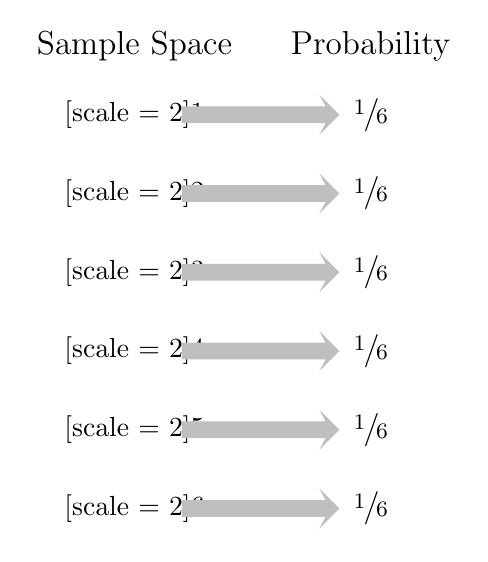
\begin{tikzpicture}
	\foreach \n in {1,...,6} {
		\node at ($(0,7)-(0,\n)$) {\drawdie [scale = 2]{\n}};
		\node [fill=gray!50,
		       minimum height = 2cm,
		       minimum width = 0.1cm,
		       single arrow,
		       single arrow head extend =.15cm,
		       single arrow head indent =.08cm,
		       inner sep=1mm] at ($(1.55,7)-(0,\n)$) {};
		\node  (p1) at (3,\n) {\large{$\sfrac{\text{1}}{\text{6}}$}};
	}
	\node [text centered,
	       anchor=south,
	       text height = 1.5ex,
	       text depth = .25ex] (p3) at (0,6.6) {\large{{Sample Space}}};
	\node [text centered,
	       anchor = south,
	       text height = 1.5ex,
	       text depth = .25ex] (p4) at (3,6.6) {\large{{Probability}}};
	\end{tikzpicture}	
\end{document}